% 2010 年山东卷理科第 21 题：椭圆、等轴双曲线与点 P。
% 来源 PDF：普通高考/2010/2010山东理.pdf，SHA-256 c0298cae8fcf19d5f6343a7257702c03f2b618318b10d2340f0c9cc3d67d61f5。
% 原页：第 2 页（A3 三栏）第 2 栏上部，书页码 620。
% 重绘依据：椭圆 x^2/8+y^2/4=1，双曲线 x^2/4-y^2/4=1；
%   F1(-2,0)、F2(2,0)，P(4,√12) 在双曲线上；PF1、PF2 与椭圆交于 A、B、C、D。
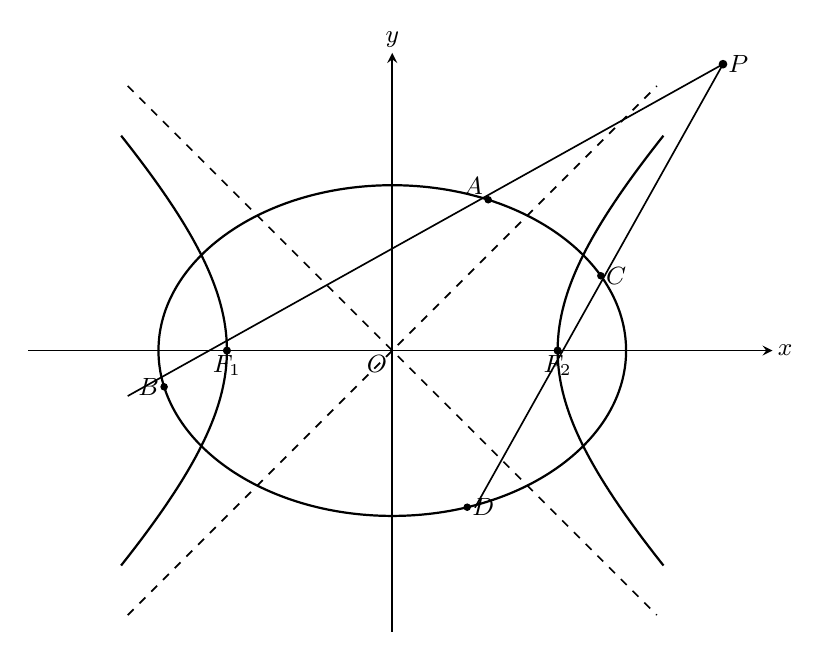
\begin{tikzpicture}[semithick, scale=1.05, every node/.style={inner sep=1.6pt, font=\small}]
  \draw[-stealth] (-4.4,0) -- (4.6,0) node[right] {$x$};
  \draw[-stealth] (0,-3.4) -- (0,3.6) node[above] {$y$};
  \draw[thick] (0,0) ellipse (2.828 and 2);
  \draw[thick,domain=-2.6:2.6,samples=80] plot ({sqrt(4+\x*\x)},\x);
  \draw[thick,domain=-2.6:2.6,samples=80] plot ({-sqrt(4+\x*\x)},\x);
  \draw[dashed] (-3.2,-3.2) -- (3.2,3.2);
  \draw[dashed] (-3.2,3.2) -- (3.2,-3.2);
  \fill (-2,0) circle (1.4pt) node[below] {$F_1$};
  \fill (2,0) circle (1.4pt) node[below] {$F_2$};
  \fill (4,3.4641) circle (1.5pt) node[right] {$P$};
  \draw (4,3.4641) -- (-3.2,-0.55);
  \draw (4,3.4641) -- (1.0,-1.9);
  \fill (1.1596,1.8242) circle (1.3pt) node[above left] {$A$};
  \fill (-2.7596,-0.4386) circle (1.3pt) node[left] {$B$};
  \fill (2.5224,0.9048) circle (1.3pt) node[right] {$C$};
  \fill (0.9062,-1.8946) circle (1.3pt) node[right] {$D$};
  \node[below left] at (0,0) {$O$};
\end{tikzpicture}
